\documentclass[11pt]{scrartcl}
\usepackage[utf8]{inputenc}
\usepackage{mathtools}
\usepackage{amssymb}
\usepackage{listings}
\usepackage{bm}
\usepackage{array}
% \usepackage{graphicx}
% \usepackage{xcolor}
% \usepackage{qtree}
% \usepackage{tikz}
\lstset
{ %Formatting for code in appendix
    language=Matlab,
    basicstyle=\footnotesize,
    numbers=left,
    stepnumber=1,
    showstringspaces=true,
    tabsize=1,
    breaklines=true,
    breakatwhitespace=false,
}
\begin{document}
\centerline{\LARGE{\textbf{CSE881 HW9}}}
\centerline{\large{\textit{Nan Cao,\  A52871775}}}
\centerline{\large{\textit{Nov 20th, 2016}}}

\section*{Problem 1}
% \begin{equation*}
% \begin{aligned}
% \begin{bmatrix}
%    & P1     & P2     & P3     & P4     & P5    \\
% P1 & 0      & 0.5840 & 0.1955 & 0.3815 & 0.1127\\
% P2 & 0.5840 & 0      & 0.6132 & 0.4956 & 0.5733\\
% P3 & 0.1955 & 0.6132 & 0      & 0.2390 & 0.3067\\
% P4 & 0.3815 & 0.4956 & 0.2390 & 0      & 0.4694\\
% P5 & 0.1127 & 0.5733 & 0.3067 & 0.4694 & 0     \\
% \end{bmatrix}
% \end{aligned}
% \end{equation*}
\begin{figure}[h]
    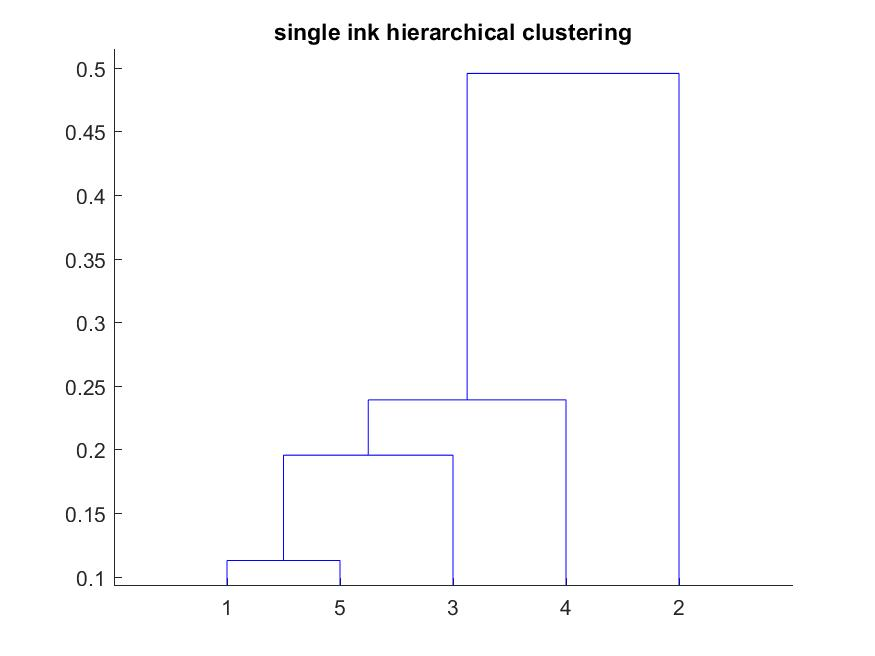
\includegraphics[width=4.5in,height=3in]{q1single.jpg}
\end{figure}
\begin{figure} [h]
    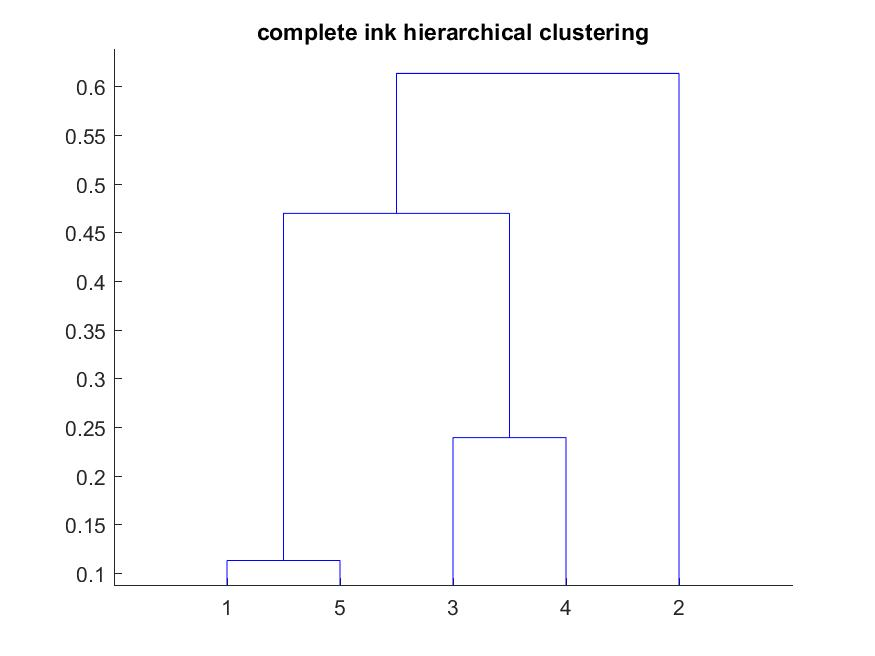
\includegraphics[width=4.5in,height=3in]{q1complete.jpg}
\end{figure}
\section*{Problem 2}
\textbf{(a)}\\
a,b,c,d,e,f,g,h,i,j,k;\\
m,o,p,q,r,s,t,u,v,w,x\\
\textbf{(b)}\\
l,n,y\\
\textbf{(c)}\\
z\\
\textbf{(d)}\\
2 clusters will be ontained.\\
\section*{Problem 3}
\textbf{(a)}\\
\begin{equation*}
\begin{aligned}
\mathbf{W}=&
\begin{bmatrix}
0 & 1 & 1 & 0 & 0 & 0 & 0\\
1 & 0 & 1 & 0 & 0 & 0 & 0\\
1 & 1 & 0 & 1 & 0 & 0 & 0\\
0 & 0 & 1 & 0 & 0 & 1 & 0\\
0 & 0 & 0 & 0 & 0 & 1 & 1\\
0 & 0 & 0 & 1 & 1 & 0 & 1\\
0 & 0 & 0 & 0 & 1 & 1 & 0\\
\end{bmatrix}\\
\mathbf{D}=&
\begin{bmatrix}
2 & 0 & 0 & 0 & 0 & 0 & 0\\
0 & 2 & 0 & 0 & 0 & 0 & 0\\
0 & 0 & 3 & 0 & 0 & 0 & 0\\
0 & 0 & 0 & 2 & 0 & 0 & 0\\
0 & 0 & 0 & 0 & 2 & 0 & 0\\
0 & 0 & 0 & 0 & 0 & 3 & 0\\
0 & 0 & 0 & 0 & 0 & 0 & 2\\
\end{bmatrix}\\
\mathbf{L}=\mathbf{D}-\mathbf{W}=&
\begin{bmatrix}
 2 &-1 &-1 & 0 & 0 & 0 & 0\\
-1 & 2 &-1 & 0 & 0 & 0 & 0\\
-1 &-1 & 3 &-1 & 0 & 0 & 0\\
 0 & 0 &-1 & 2 & 0 &-1 & 0\\
 0 & 0 & 0 & 0 & 2 &-1 &-1\\
 0 & 0 & 0 &-1 &-1 & 3 &-1\\
 0 & 0 & 0 & 0 &-1 &-1 & 2\\
\end{bmatrix}\\
\end{aligned}
\end{equation*}
\textbf{(b)}\\
\begin{equation*}
\begin{aligned}
\mathbf{\lambda}=&
\begin{bmatrix}
0& 0& 0& 0& 0& 0& 0\\
& 0&0.2679& 0& 0& 0& 0& 0\\
& 0& 0&1.5858& 0& 0& 0& 0\\
& 0& 0& 0&3& 0& 0& 0\\
& 0& 0& 0& 0&3& 0& 0\\
& 0& 0& 0& 0& 0&3.7321& 0\\
& 0& 0& 0& 0& 0& 0&4.4142\\
\end{bmatrix}\\
\mathbf{V}=&
\begin{bmatrix}
& 0.3780&-0.4440&-0.2808& 0.7071& 0.0020& 0.2299&-0.1683\\
& 0.3780&-0.4440&-0.2808&-0.7071&-0.0020& 0.2299&-0.1683\\
& 0.3780&-0.3251& 0.1645&-0.0000& 0.0000&-0.6280& 0.5745\\
& 0.3780&-0.0000& 0.7941&-0.0000& 0.0000& 0.0000&-0.4760\\
& 0.3780& 0.4440&-0.2808& 0.0020&-0.7071&-0.2299&-0.1683\\
& 0.3780& 0.3251& 0.1645& 0.0000&-0.0000& 0.6280& 0.5745\\
& 0.3780& 0.4440&-0.2808&-0.0020& 0.7071&-0.2299&-0.1683\\
\end{bmatrix}
\end{aligned}
\end{equation*}
$$\mathbf{\lambda}=(0,
    0.2679,
    1.5858,
    3,
    3,
    3.7321,
    4.4142)^{T}$$
The smallest three eigenvalues:\\
$$\lambda_{(1)}=0,\lambda_{(2)}=1.5858,\lambda_{(3)}=3$$
\textbf{(c)}
\begin{equation*}
\begin{aligned}
 \mathbf{e}_{(1)}=&  
   (0.3780,
    0.3780,
    0.3780,
    0.3780,
    0.3780,
    0.3780,
    0.3780)^T\\
    \mathbf{e}_{(2)}=&  
  (-0.4440,
   -0.4440,
   -0.3251,
   -0.0000,
    0.4440,
    0.3251,
    0.4440)^T\\
    \mathbf{e}_{(3)}=&  
  (-0.2808,
   -0.2808,
    0.1645,
    0.7941,
   -0.2808,
    0.1645,
   -0.2808)^T\\
\end{aligned}
\end{equation*}
\textbf{(d)}\\
\begin{center}
\begin{tabular}{| p{1.75cm}| p{0.75cm}| p{0.75cm}| p{0.75cm}| p{0.75cm}| p{0.75cm}| p{0.75cm}| p{0.75cm}|}
    \hline
    EigVec&$\mathbf{e}_1$&$\mathbf{e}_2$&$\mathbf{e}_3$&$\mathbf{e}_4$&$\mathbf{e}_5$&$\mathbf{e}_6$&$\mathbf{e}_7$\\
    \hline
    Cluster&1&1&1&2&3&3&3\\
    \hline
\end{tabular}\\
\{$\mathbf{e}_1$,$\mathbf{e}_2$,$\mathbf{e}_3$\};
\{$\mathbf{e}_4$\};
\{$\mathbf{e}_5$,$\mathbf{e}_6$,$\mathbf{e}_7$\};\\
\end{center}
\textbf{(e)}\\
\begin{equation*}
\begin{aligned}
Ncut(V_1,V_2,V_3)=&
\frac{Cut(V_1,V-V_1)}{d(V_1)}
+\frac{Cut(V_2,V-V_2)}{d(V_2)}
+\frac{Cut(V_3,V-V_3)}{d(V_3)}\\
=&\frac{2}{7}+1+\frac{2}{7}\\
=&\frac{11}{7}\\
\end{aligned}
\end{equation*}
\textbf{(f)}\\
\begin{equation*}
\begin{aligned}
Ncut(V_1,V_2,V_3)=&
\frac{Cut(V_1,V-V_1)}{d(V_1)}
+\frac{Cut(V_2,V-V_2)}{d(V_2)}
+\frac{Cut(V_3,V-V_3)}{d(V_3)}\\
=&\frac{2}{4}+\frac{4}{8}+\frac{2}{4}\\
=&\frac{3}{2}\\
\end{aligned}
\end{equation*}
It's larger than the solution found in (d).
\end{document}

% \begin{equation*}
% \begin{aligned}
% \end{aligned}
% \end{equation*}\\